The Android \gls{sdk} provides useful tools regarding the development and study of Android apps. It is the case of the \textit{emulator}, placed at \texttt{tools/} and the \gls{adb}, placed at \texttt{platform-tools/}. This section describes both tools regarding their valuable features to this project.

\subsection{Android Emulator}

Android supplies a mobile device emulator based on the Qemu virtual machine that runs on the computer. This emulator provides a real Android environment, being able to run any application. It is very useful to developers, because avoids the need of having a real device in order to run applications. However, depending on the computer's characteristics, the performance of the Android emulator may be considerable low when compared to real devices.

\begin{figure}[h]
 \centering
 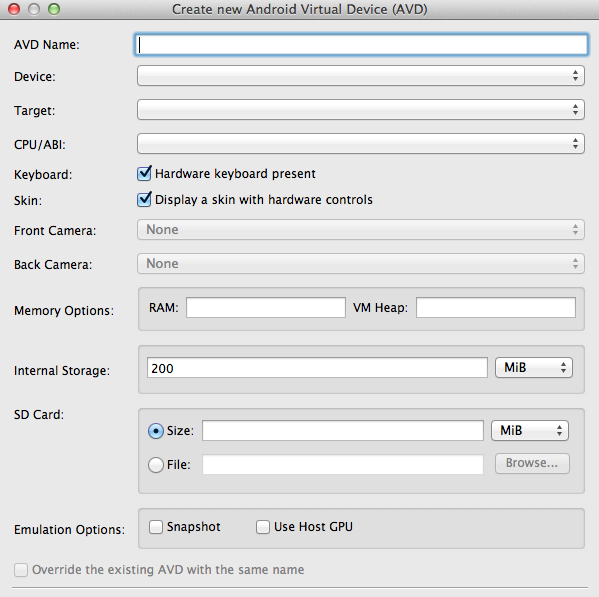
\includegraphics[scale=0.5]{figures/avd.png}
 \caption{Android Virtual Device configuration}
 \label{fig:avd}
\end{figure}

The Android emulator boots an Android image according to the \gls{avd} configuration file. The \gls{avd} allows to define hardware and software characteristics of a specific model to run on the Android emulator. \autoref{fig:avd} shows a snapshot of the \gls{avd} window configuration. For instance, in the \textit{Device} option it is possible to choose an Android model, as \textit{Nexus 4}, \textit{Nexus 7}, \textit{Nexus 10}, \textit{Galaxy Nexus}, \textit{Nexus S}, etc. The \textit{Target} element defines the Android version and the corresponding \gls{api}, as \textit{Android 2.3.3 - API Level 10}, \textit{Android 4.4 - API Level 19}, etc.

Once the \gls{avd} is created, the emulator may be launched through the \gls{avd} Manager or using the command line. Some useful commands\footnote{http://developer.android.com/tools/help/emulator.html} are presented as follow.

\begin{lstlisting}[caption=Command to start the Android emulator]
# emulator -avd <avd_name>
\end{lstlisting}

This command launches the emulator with the \gls{avd} image called \textt{avd\_name}. \gls{avd} files are usually stored at \texttt{.android/avd/} within the Android \gls{sdk} folder.

\begin{lstlisting}[caption=Command to provide a kernel to the Android emulator]
# emulator -avd <avd_name> -kernel <kernel_path>
\end{lstlisting}

In order to choose a kernel of our own, to run on the emulator, it is used the \texttt{-kernel} flag followed by the path of the image kernel file.

 \begin{lstlisting}[caption=Command to provide kernel prints of the Android emulator]
# emulator -avd <avd_name> -kernel <kernel_path> -show-kernel -verbose
\end{lstlisting}

To follow what is happening during the boot and to inspect kernel prints, the emulator provides both \texttt{-show-kernel} and \texttt{-verbose} flags.

\subsection{Android Debug Bridge}

\gls{adb}\footnote{http://developer.android.com/tools/help/adb.html} is another useful tool that connects the computer to Android devices (real or emulated). This connection brings powerful features that will be described in this section. The \gls{adb} tool, mention as adb from now on, is available as a command line. It is a client-server program that comprises three components:

\begin{itemize}
\item A client, that runs on the development computer;
\item A server, that runs as a background process on the development computer. The server handles communication between the client and the daemon;
\item A daemon, that runs in background on the mobile device (real or emulated).
\end{itemize}

Once Android emulator is started, adb provides a means of communication. The following command shows all Android devices running on the computer:

 \begin{lstlisting}[caption=Command to show Android devices running on the computer]
# adb devices
\end{lstlisting}

If there is an Android emulator running on the computer, the output returned is similar to the following:

 \begin{lstlisting}[caption=Example of the output from the \texttt{adb devices} command]
List of devices attached 
emulator-5554	device
\end{lstlisting}

With adb it is possible to:

\begin{itemize}

\item install an Android application on the emulator/device;
 \begin{lstlisting}[caption=Command to install Android apps using the adb utility]
# adb install <path_to_apk>
\end{lstlisting}

\item copy a specific file from the emulator/device to the development computer;
 \begin{lstlisting}[caption=Command to pull files using the adb utility]
# adb pull <remote> <local>
\end{lstlisting}

\item copy a specific file from the development computer to the emulator/device;
 \begin{lstlisting}[caption=Command to push files using the adb utility]
# adb push <local> <remote>
\end{lstlisting}

\item print the logcat output;
 \begin{lstlisting}[caption=Command to get logcat's prints using the adb utility]
# adb logcat
\end{lstlisting}

\item start a remote shell in the target emulator/device:
 \begin{lstlisting}[caption=Command to start a remote shell using the adb utility]
# adb shell
\end{lstlisting}

\end{itemize}

There are more options to execute with adb that can be checked on the Android online page\footnote{http://developer.android.com/tools/help/adb.html}.